% !TeX program = PdfLaTeX
% !TeX root = ../Elaborati_Aerodinamica_Bruno_Spoti.tex
\chapter{Generalità e geometria del profilo alare PW106}

Il seguente lavoro si prefigge lo scopo di studiare le prestazioni aerodinamiche del profilo alare {\bfseries PW106}, un profilo disegnato da Peter Wick e ottenuto a partire dal profilo alare simile PW51 rispetto al quale ha una curvatura maggiore e quindi un maggiore $C_{l_\mathrm{MAX}}$. 
La valutazione delle caratteristiche dello stesso è stata condotta attraverso l'applicazione di metodi teorici tramite il codice XFOIL e con l'ausilio di script implementati in MATLAB.
\\
Preliminarmente è stata trattata la geometria del profilo, la cui costruzione è stata fatta per punti. In seguito sono state ricavate le caratteristiche geometriche dello stesso e i risultati del profilo sottile. È stata poi studiata la soluzione in campo Euleriano incomprimibile a vari $C_l$ significativi, graficandone il coefficiente di pressione. Si è passati, poi, alla soluzione in campo viscoso introducendo gli effetti del numero di Reynolds e della turbolenza asintotica. Sono stati inoltre valutati gli effetti sullo strato limite in condizioni di alta portanza verificando, in base ai criteri semiempirici, il tipo di stallo del profilo in esame. Infine é stata ricavata l'aerodinamica del profilo considerando la deflessione di parte dello stesso come {\itshape flap} oppure come alettone.

\section{Geometria del Profilo}

La geometria del profilo è stata inizialmente fornita in forma tabellare con 33 punti sul dorso e 29 sul ventre \cite{prof:sito}. \\ 

%GRAFICO PROFILO PUNTI S4110


\begin{figure} [h!]
\centering
\begin{tikzpicture} 
\begin{axis} [ 
xmin=0, 
xmax=1, 
ymin=-0.1,
 ymax=0.1,
 xlabel=$ \frac {x}{c}$, 
ylabel=$ \frac {z}{c}$,
ytick={-0.1,-0.05,0,0.05,0.1},
yticklabels={$-0.1$,$-0.05$,$0$,$0.05$,$0.1$},
width=13cm,
 height=2.6 cm,
scale only axis,
grid=major] 
\addplot [black, mark=*,only marks]
file{images/profilopw106.dat};
\end{axis}
\end{tikzpicture}
\caption{\footnotesize Profilo alare PW106. Punti assegnati (33 sul dorso, 29 sul ventre) }\label{fig:cp}
\end{figure}
\noindent
 \\ 


 La disegnazione tecnica del profilo e le successive applicazioni sono state condotte su una geometria migliorata tramite Spline, al fine di evitare spigolositá o salti nei grafici del coefficiente di pressione.\\ 

%GRAFICI PROFILO

\begin{figure} [h!]
\centering
\begin{tikzpicture} 
\begin{axis} [ 
xmin=0, 
xmax=1, 
ymin=-0.1,
 ymax=0.1,
 xlabel=$ \frac {x}{c}$, 
ylabel=$ \frac {z}{c}$,
ytick={-0.1,-0.05,0,0.05,0.1},
yticklabels={$-0.1$,$-0.05$,$0$,$0.05$,$0.1$},
width=13cm,
 height=2.6 cm,
scale only axis,
grid=major] 
\addplot [black,solid,very thick]
file{immagini/s4110tretretre3.dat};
\addplot [black,solid,very thick]
file{immagini/lineamedia.dat};
\end{axis}
\end{tikzpicture}
\caption{\footnotesize Profilo alare S4110. Geometria migliorata con Spline }\label{fig:cp}
\end{figure}
\noindent
 \\ \\


\begin{figure} [h!]
\centering
\begin{tikzpicture} 
\begin{axis} [ 
xmin=0, 
xmax=1, 
ymin=-0.1,
 ymax=0.1,
 xlabel=$ \frac {x}{c}$, 
ylabel=$ \frac {z}{c}$,
ytick={-0.1,-0.05,0,0.05,0.1},
yticklabels={$-0.1$,$-0.05$,$0$,$0.05$,$0.1$},
width=13cm,
 height=2.6 cm,
scale only axis,
grid=major] 
\addplot [black,solid,very thick]
file{immagini/s4110tretretre3.dat};
\addplot [black,solid,very thick]
file{immagini/lineamedia.dat};
\addplot [black, mark=*,thick]
file{immagini/s4110.dat};
\end{axis}
\end{tikzpicture}
\caption{\footnotesize Profilo alare S4110.Confronto punti assegnati - geometria spline }\label{fig:cp}
\end{figure}
\noindent
 \\ \\

\begin{figure} [h!]
\centering
\begin{tikzpicture} 
\begin{axis} [ 
xmin=-0.03, 
xmax=0.1, 
ymin=-0.03,
 ymax=0.05,
 xlabel=$ \frac {x}{c}$, 
ylabel=$ \frac {z}{c}$,
xtick={-0.03,0,0.03,0.06,0.09},
width=13cm,
 height=8.61 cm,
scale only axis,
grid=major] 
\addplot [black,solid,very thick]
file{immagini/s4110tretretre3.dat};
\end{axis}
\end{tikzpicture}
\caption{\footnotesize Profilo alare S4110. Zoom del bordo d'attacco }\label{fig:cp}
\end{figure}
\noindent
 \\ \\

\begin{figure} [h!]
\centering
\begin{tikzpicture} 
\begin{axis} [ 
xmin=0.9, 
xmax=1.02, 
ymin=-0.01,
 ymax=0.03,
 xlabel=$ \frac {x}{c}$, 
ylabel=$ \frac {z}{c}$,
%xtick={-0.03,0,0.03,0.06,0.09},
width=13cm,
 height=4.33 cm,
scale only axis,
grid=major] 
\addplot [black,solid,very thick]
file{immagini/s4110tretretre3.dat};
\end{axis}
\end{tikzpicture}
\caption{\footnotesize Profilo alare S4110. Zoom del bordo d'uscita }\label{fig:cp}
\end{figure}
\noindent
 \\ \\




 Al fine di migliorare la geometria, i punti di ascissa ({\bfseries X}), ordinata({\bfseries Y}) e ascissa curvilinea del profilo ({\bfseries S}),  sono stati importati in MATLAB ed elaborati con un codice in grado di generare delle {\itshape spline} X(S) e Y(S) ed interpolarle al fine di ottenere 100 punti sul dorso e 100 punti sul ventre, alle stesse ascisse.
L'interpolazione delle {\itshape spline} su uno stesso intervallo di ascisse ha consentito la disegnazione della linea media del profilo e la valutazione dello spessore in funzione dell’ascissa X lungo la corda.\\ \\

%ASCISSA- ORDINATA - ASCISSACURVILINEA 

\begin{figure} [h!]
\centering
\begin{tikzpicture} 
\begin{axis} [ 
xmin=0, 
xmax=2.02, 
ymin=0,
 ymax=1,
 xlabel=$ \frac {s}{c}$, 
ylabel=$ \frac {x}{c}$,
width=12cm,
 height=6 cm,
scale only axis,
grid=major] 
\addplot [black,solid,very thick]
file{immagini/ascissa_ascissacurvilinea.dat};
\end{axis}
\end{tikzpicture}
\caption{\footnotesize S4110- Andamento ascissa curvilinea - ascissa }\label{fig:cp}
\end{figure}
\noindent
 \\ \\

\begin{figure} [h!]
\centering
\begin{tikzpicture} 
\begin{axis} [ 
xmin=0, 
xmax=2.02, 
ymin=-0.05,
 ymax=0.1,
 xlabel=$ \frac {s}{c}$, 
ylabel=$ \frac {z}{c}$,
width=12cm,
 height=6 cm,
scale only axis,
ytick={-0.05,0,0.05,0.1},
grid=major] 
\addplot [black,solid,very thick]
file{immagini/ordinata_ascissacurvilinea.dat};
\end{axis}
\end{tikzpicture}
\caption{\footnotesize  S4110-Andamento ascissa curvilinea - ordinata}\label{fig:cp}
\end{figure}
\noindent
 \\ 

Tramite xfoil é stata ricavato l'andamento della curvatura del profilo in funzione dell'ascissa curvilinea, riportato nelle figure che seguono.\\

\begin{figure} [h!]
\centering
\begin{tikzpicture} 
\begin{axis} [ 
xmin=0, 
xmax=2.02, 
ymin=0,
 ymax=120,
 xlabel=$ \frac {s}{c}$, 
ylabel=curvatura,
width=11cm,
 height=8 cm,
scale only axis,
grid=major] 
\addplot [black,solid,very thick]
file{immagini/curvatura.dat};
\end{axis}
\end{tikzpicture}
\caption{\footnotesize S4110- Andamento ascissa curvilinea - curvatura }\label{fig:cp}
\end{figure}
\noindent
 \\ \\

\begin{figure} [h!]
\centering
\begin{tikzpicture} 
\begin{axis} [ 
xmin=0, 
xmax=2.02, 
ymin=-1,
 ymax=2,
 xlabel=$ \frac {s}{c}$, 
ylabel=curvatura,
width=11cm,
 height=7 cm,
scale only axis,
grid=major] 
\addplot [black,solid,very thick]
file{immagini/curvatura.dat};
\end{axis}
\end{tikzpicture}
\caption{\footnotesize  S4110-Andamento ascissa curvilinea - curvatura, zoom }\label{fig:cp}
\end{figure}
\noindent
 \\


Si noti come in alcuni punti del profilo, in prossimitá del bordo d'uscita, la curvatura sia negativa.\\


I punti del profilo sono stati importati sul software CAD CATIA V5 per rappresentare l’ala infinita, con profilo costante, di elevato allungamento.

\begin{figure} [h!]
\centering
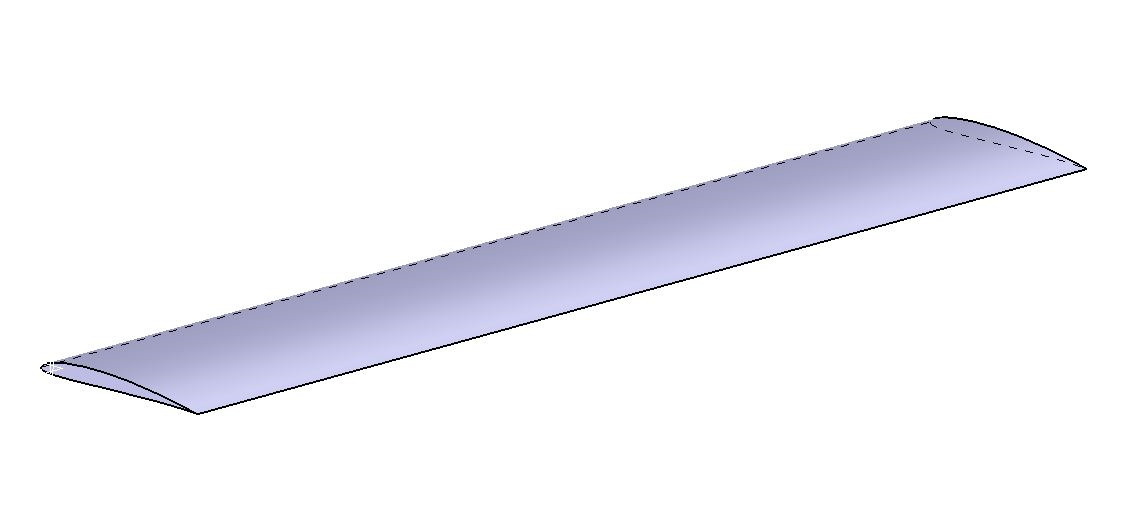
\includegraphics  [ height=6cm] {immagini/s41103.png}
\caption{\footnotesize Ala infinita, profilo costante S4110, rendering in CATIA V5}
\label{fig:catia}
\end{figure}